\documentclass{article}

\usepackage[normalem]{ulem}
\usepackage{fancyhdr}
\usepackage[parfill]{parskip}
\usepackage{tikz}
\usepackage{pgfplots}
\usepackage{multicol}
\usepackage[version=3]{mhchem}
\usepackage{multirow}
\usepackage{SIunits}
\pagestyle{fancyplain}

\pgfplotsset{compat=1.7}

\title{Capacitors}
\author{Todd Davies}
\date{\today}

\begin{document}

\rhead{Capacitors}
\lhead{\today}

\maketitle

\section*{Equations to learn}
\thispagestyle{empty}

\begin{itemize}
	
	\item The energy stored by a capacitor for a given potential difference is:
	
	\[
		W = \frac{1}{2}QV = \frac{1}{2}CV^2 = \frac{Q^2}{2C}
	\]

	\item The combined capacitance of capacitors in parallel is:

	\[
		C_{total} = C_1 + C_2 + +... + C_n
	\]

	\item The combined capacitance of capacitors in series is:
	
	\[
		\frac{1}{C_{total}} + \frac{1}{C_1} + \frac{1}{C_2} + ... + \frac{1}{C_n}
	\]

	\item The decay of charge, current or potiential difference in a capacitor
	is modelled by the equation:

	\[
		x = x_0 e^{-\frac{t}{CR}}
	\]

	\item The time constant of a capacitor is given by:

	\[
		t = CR
	\]

\end{itemize}


\section*{What are capacitors?}

Capacitors are electrical components that store charge. They are composed of two
sheets of metal seperated by a piece of insulating material called the {\it
dielectric}.

To charge the capacitor, a voltage is applied across it. The negative terminal
pushes electrons onto one plate, and the positive terminal pulls them off the
other. Since there is an insulator between the plates, the electrons cannot
cross the gap and there is a charge difference between the plates (even though
the net charge is zero).

When the capacitor is then connected to a circuit, the electrons flow out of the
negative terminal towards the positive terminal, powering the circuit.

\section*{What is capacitance}

Capacitance is the charge stored for a g qiven potiential difference. In
equation form:

\[
	C = \frac{Q}{V}
\]

The units of capacitance are the Farad (F), which is equal to one Columb per
Volt ($CV^{-1}$).

\section*{Energy stored in a capatitor}

You can work out the (small) amount of energy in capacitors by using the
equation:

\[
	W = \frac{1}{2}CV^2
\]

If you look carefully at this graph, you will be able to see that the area under
a potential difference against charge graph is equal to the energy stored by the
capacitor.

For any one capacitor, we can also work out the relationship between energy
stored and charging voltage of the capacitor by taking out some constants:

\[
	W \propto V^2
\]

\section*{Capacitors in parallel}

When capacitors are placed in parallel, they are electrically just one big
capacitor, since all their plates are electrically joined.

Hence the equation for the total charge stored is $Q = C_{total}V$, the
potiential difference is the same across all of them, the total charge across
them is equal to the sum of their charges ($Q_{total} = Q_1 + Q_2 + ... + Q_n$)
and the equation for the total capacitance is $C_{total} = C_1 + C_2 + ... +
C_n$.

\section*{Capacitors in series}

The total capacitance of capacitors in series is given by the equation:

\[
	\frac{1}{C_{total}} = \frac{1}{C_1} + \frac{1}{C_2} + ... + \frac{1}{C_n}
\]

However, it is important to remember that the potiential difference across all
of the capacitors is given by:

\[
	V_{total} = V_1 + V_2 + ... + V_n
\]

\section*{Capacitors and resistors}

Learn this table:

\def\arraystretch{1.5}
\begin{tabular}{|l|l|l|}
	\hline
	& {\bf Capacitors} & {\bf Resistors} \\ \hline

	\multirow{2}{*}{\bf In series} & All store the same charge & All have the 
	same current \\
	& $\frac{1}{C_{total}} = \frac{1}{C_1} + \frac{1}{C_2} + ... + 
	\frac{1}{C_n}$ & $R_{total} = R_1 + R_2 + ... + R_n$\\ \hline

	\multirow{2}{*}{\bf In parallel} & All have the same p.d & All have the same
	p.d \\
	& $C_{total} = C_1 + C_2 + ... + C_n$ & 
	$\frac{1}{R_{total}} = \frac{1}{R_1} + \frac{1}{R_2} + ... +
	\frac{1}{R_n}$\\ \hline

\end{tabular}

\section*{Solving problems about capacitor networks}

In order to solve problems related to capacitor networks, first attempt to
recursivly break seperate the circuit diagram up into sections, and then list
the qualities of each section.

\newpage

Take this circuit diagram for example:

\begin{center}
	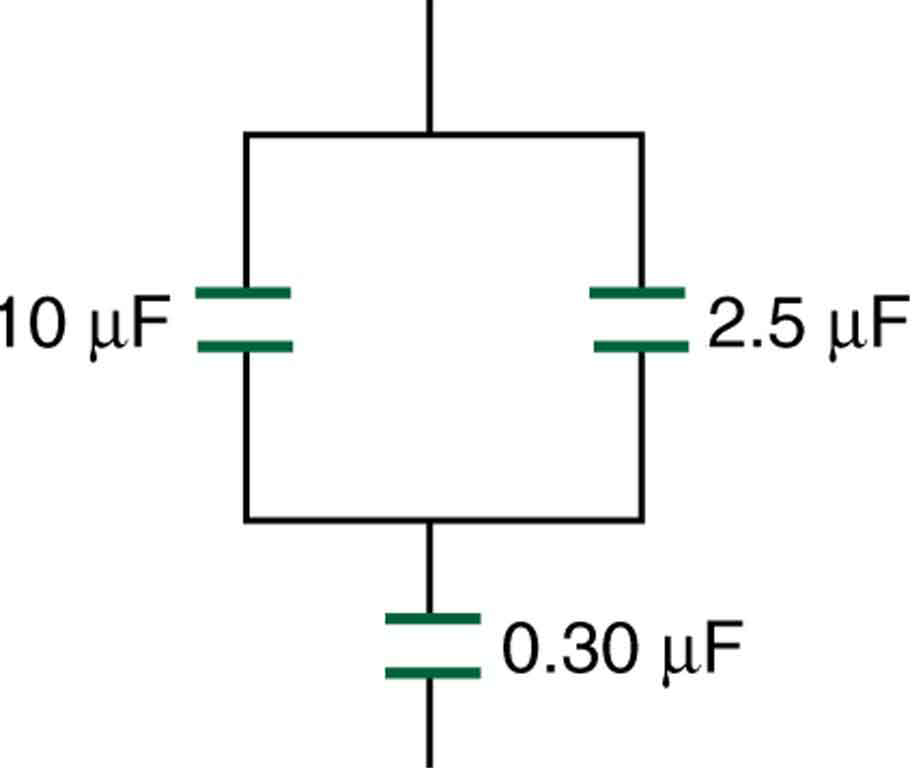
\includegraphics[height=6cm, width=6cm]{diagram}
\end{center}

In order to find the total capacitance of the network, we must break it down
into two parts, the top two resistors in parallel, and the bottom resistor in
series.

First we find the combined capacitance of the top two capacitors and then sub
that into the equation for the capacitance of capacitors in series.

\[
	C_{total} = \frac{1}{ \frac{1}{10 + 2.5} + \frac{1}{0.30} } = 0.293\micro\farad
\]

\section*{Discharging capacitors}

The graph of a capacitor discharge displays an exponiential decay. The time
taken for a capacitor to lose half of it's charge is called the {\bf time
constant}.

The reason this occurs with capacitors is because initially, when the capacitor
is charged up, all the electrons on one plate repel each other. When it is
allowed to discharge, as the charge on the capacitor decreases,  the p.d. also
decreases and so the current decreases. Concequently, the charge, p.d. and
current all decrease more slowly, giving us the exponiential curve displayed on
the graph.

The charge, current or p.d of the capacitor at any time $t$ can be found using
the equation:

\[
	X = X_0e^{-\frac{t}{CR}}
\]

Where $X$ is either the charge, current or p.d., $t$ is the time taken from the
start of the discharge, $C$ is the capacitance of the capacitor and $R$ is the
resistance of the circuit.

\subsubsection*{Example}

A $1000\micro\farad$ capacitor initially stores $20\milli\coulomb$ of charge. It
is discharged through a resistor of resistance $500\kilo\ohm$. Calculate the
charge left on the capacitor after $100\second$.

{\bf Step 1} - write down the values in standard form

$Q_0 = 20\milli\coulomb = 20\times10^{-3}\coulomb$

$t = 100\second$

$C = 1000\micro\farad = 1000\times10^{-6}\farad$

$R = 500\kilo\ohm = 500\times10^3\ohm$

{\bf Step 2} - Calculate $Q$ using $X = X_0e^{-\frac{t}{CR}}$

$Q = 20\times10^{-3}e^{-\frac{100}{1000\times10^{-6} \times 500\times10^3}}$

$Q = 20\times10^{-3}e^{-0.2}$

$Q = 1.64\times10^{-2}\coulomb$

$Q = 16.4\milli\coulomb$

\section*{Time constant $\tau$}

The time constant of a capacitor is equal to the product of it's capacitance and
the resistance across it's terminals.

\[
	\tau = CR
\]

This is because:

\begin{itemize}

	\item With larger values of the capacitance C, more charge can be stored and
	it takes longer to drain the capacitor.

	\item With larger values of the resistance R, the current will be smaller,
	causing the capacitor to take more time to discharge.

\end{itemize}

The time constant is defined as:

{\it The time taken for the current, charge stored, or potential difference to
fall to $\frac{1}{e}$ (or 37\%) of it's initial value.}

Although in theory, it takes an infinate amount of time for a capacitor to fully
discharge, in practice, capacitors are said to have fully discharged after a
time of $5\tau$.

\section*{Questions}

\subsection*{Question 1}

A $100\micro\farad$ capacitor is charged to $6\volt$. It is then discharged
through a resistor of resistance $500\kilo\ohm$.

{\bf a)} Calculate the time constant.

{\bf b)} Calculate the current after $1\minute$.

\subsection*{Answer 1}

\paragraph{a)}
\setlength\parindent{20pt}
$\tau = CR$

$\tau = 100\times10^{-6} \times 500\times10^3$

$\tau = 50\second$

\paragraph{b)}
\setlength\parindent{20pt}

$I = I_0e^{-\frac{t}{CR}}$

$V=IR$

$6 = 500\times10^3 \times I_0$

$I_0 = 1.2\times10^{-5}\ampere$

$I = 1.2\times10^{-5}e^{-\frac{60}{50}}$

$I = 3.6\times10^{-6}$ 

\subsection*{Question 2}

Calculate the current required to charge a $50\micro\farad$ capacitor to a p.d.
of $10\volt$ in a time of $0.01\second$.

\subsection*{Answer 2}
\setlength\parindent{0pt}
$C = \frac{Q}{V}$

$Q = 50\times10^{-6}\times10 = 5\times10^{-4}$

$\frac{5\times10^{-4}}{0.01} = 0.05\ampere$

\end{document}